%location/filename: tex/ch1.tex
%author: Anders Østevik
% Created: 28.2.2016
%#######--Chapter 4--#######
%Content:	

\documentclass[main.tex]{subfiles}

%\usetikzlibrary{arrows,automata}

\begin{document}

\chapter{External and Internal Loopback test of the GBT bank Quartus Example}

\section{120 MHz reference clock}

To be able to conduct a proper loopback test, the \gls{mgt} and the \glspl{pll} of the \gls{gbt} \todo{name the proper plls and state why 120 mhz is really needed} must have a input clock frequency of $120~\mega\hertz$. There are a number of ways to achieve this on the Cyclone V board: 
\begin{itemize}
\item Using an external clock, like a differential square wave signal generator.
\item Using an on-board programmable oscillator.
\item Implementing a \gls{pll} into the design that multiplies the on-board $50~\mega\hertz$ global clock up to the desired frequency of $120~\mega\hertz$.
\end{itemize}

The original approach is to use an external signal generator to generate the reference clock, as shown in the \gls{gbt} tutorial videos \cite{gbt_videos}. However, at the time of conducting the first tests, there was no available signal generators that could generate a $120~\mega\hertz$ square wave clock for the experiment. Because of this, some time was spent to investigate how to use the internal programmable oscillator as a reference clock.\\

The approach of implementing an extra \gls{pll} into the \gls{gbt}-example design was also investigated, but attempts of doing so resulted in conflicts between the already implemented transceiver \glspl{pll} in the design. \\

The below sections gives the following descriptions:
\begin{itemize}
\item How to setup the internal oscillator on the Cyclone V \gls{fpga} board for use as reference clock.
\item How to setup the $Si338$ external oscillator for use as reference clock.
\end{itemize}

\subsection{Configuring the on-board oscillator on the Cyclone V board}

To achieve a reference clock of $120~\mega\hertz$ without an external clock, the \gls{fpga} has an on-board programmable oscillator; the $Si570$ from Silabs. It uses \gls{iic} for serial communication and can be programmed to output frequencies up to $810~\mega\hertz \pm 50 ppm$. To program the oscillator, Altera provides a dedicated software called "Clock Control". The Clock Control software is part of the Java based "Board Test System" software, included in the Cyclone V kit which can be found at Altera's websites \cite{altera_cyclonekit}. The Cyclone V kit is board specific, so it is therefore important to use the right kit with the right board.\\

To make use of the Clock Control software has been proven difficult, mainly because of the software being outdated in relevance to the current version of Quartus (at the time of writing, Quartus 15.0 is the newest edition). The solution was to install an older Quartus (version 13.1) using the Windows Operating System (Linux was also attempted, but without any success) and specify the right paths for the related environment variables. The below sections gives a brief description on how this was achieved.\\

\subsection{Clock Control software setup}

The Cyclone V kit is dependent on a number of Quartus related files, including the USB Blaster II device driver, the jtagconfig software and various device libraries included in the Quartus environment. It is therefore important to have the right version of Quartus installed for the Clock Control program to work properly. The version number of the kit (13.0.0.1 at the time of writing) corresponds to the supported version of Quartus, in this case Quartus 13.x (newer versions of Quartus have not proven to be backwards compatible with the Cyclone V kit).\\

By using Windows, the following steps have been proven to be the best approach to make the Clock Control software work properly. The installed path to Quartus is in this case: \path{D:\Quartus_13.1}.\\

\subsubsection{Steps for configuring Windows to run the Clock Control software}

\begin{enumerate}
  \item Install Quartus 13.x (includes jtagconfig) together with the Cyclone V device support \cite{altera_q13}.
  \item Set appropriate environment variables. In Windows, this should be set automatically.
  \begin{itemize}
      \item PATH -- \path{"D:\Quartus_13.1"}
      \item QUARTUS\_ROOTDIR -- \path{"D:\Quartus_13.1\quartus"}
      \item SOPC\_KIT\_NIOS2 -- \path{"D:\Quartus_13.1\nios2eds"}
    \end{itemize}
  \item Connect the \gls{fpga} board to the \gls{pc} using USB Blaster II (Refer to the manual for instructions on how to install the USB Blaster II \cite{altera_usb}).
  \item In Command Prompt (cmd.exe):
  \begin{itemize}
      \item Navigate to the "board\_test\_system" folder located inside the Cyclone V kit.
      \item run "jtagconfig" and confirm connection with the board. If the Command Prompt cannot find jtagconfig, navigate to \path{D:\Quartus_13.1\quartus\bin} using a file explorer and manually start jtagconfig.exe from there
      \item run "java -Djava.library.path=\path{"D:\Quartus\_13.1\bin"} -jar clk\_cont.jar". The library path is to ensure that the Java environment have access to the appropriate Quartus libraries it needs to connect with the board.
    \end{itemize}
\end{enumerate}

If done correctly, the Clock Control software will start up and display "Connected to the target" in the message window. The default output frequency of the $Si570$ oscillator is $100~\mega\hertz$. The output frequency is calculated using the following equation:

\begin{equation}
%\[
    f_{out} = \frac{f_{XTAL} \times RFREQ}{HSDIV \times N1}
%\]
\end{equation} 

, where $f_{XTAL}$ is a fixed frequency of $114,2857~\mega\hertz$; RFREQ is a floating point 38-bit word; and HSDIV and N1 is the output dividers \cite{si570}. The parameters are determined by the Clock Control software based on the user typed frequency. The parameters are then sent serially via the USB Blaster II to the $Si570$ chip, where the above formula is used to set the internal registers for the new frequency.
Figure \ref{fig:clk_cont120} shows the Clock Control software after a new frequency of $120~\mega\hertz$ is set. 

\begin{figure}[ht] % H(strictly put HERE > h!)
\begin{center}
% h(here), !(force), t(top), b(bottom), p(on extra page)
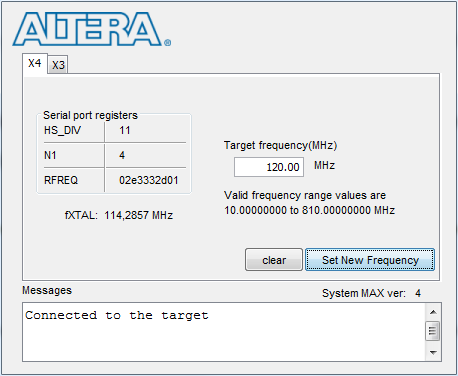
\includegraphics[scale=1]{../img/clk_cont120}  \\[0.1 cm]
\caption{Clock Control software by Altera used to program the $Si570$.}
\label{fig:clk_cont120}
\end{center}
\end{figure} 

The $Si570$ is volatile, meaning that the output frequency is reset back to $100~\mega\hertz$ if power is lost. The procedure must therefore be repeated every time the \gls{fpga} is powered on.\\
To confirm correct operation, a quick measurement of the output clock was done using an oscilloscope. Figures \ref{fig:tek100} and \ref{fig:tek120} shows the output frequency, before and after configuration.\\

\begin{figure}[!ht]
   \begin{floatrow}
     \ffigbox{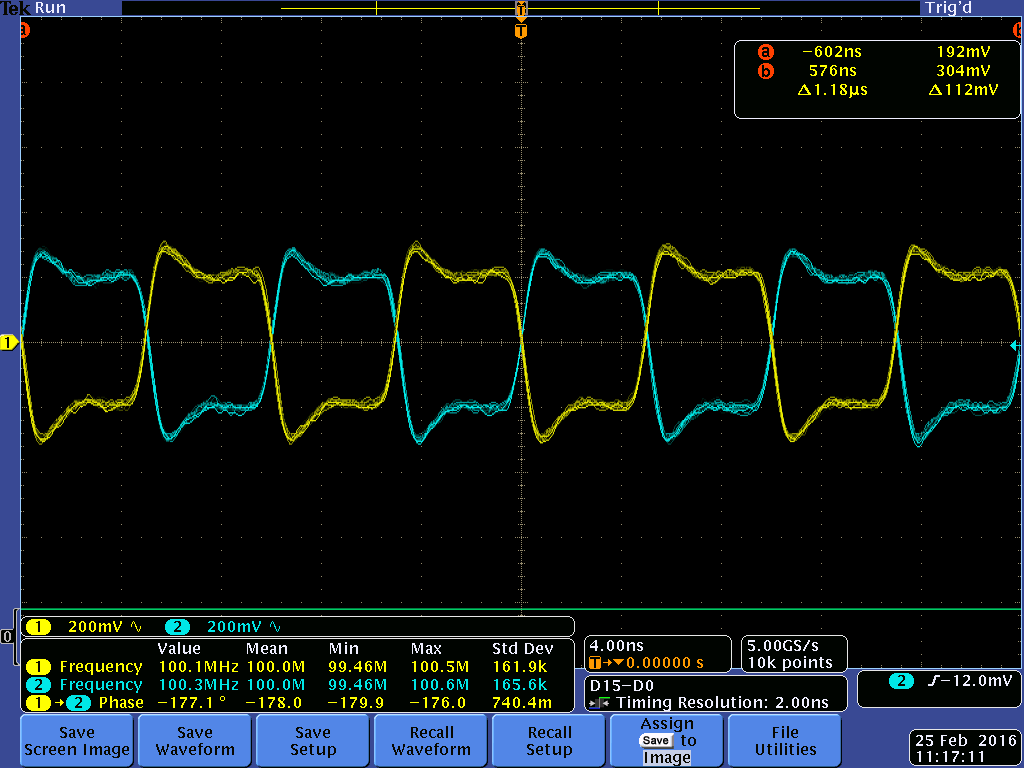
\includegraphics[scale = 0.2]{../img/20160226_tek100}}{\caption{$Si570$ Before configuration: 100 MHz.}\label{fig:tek100}}
     \ffigbox{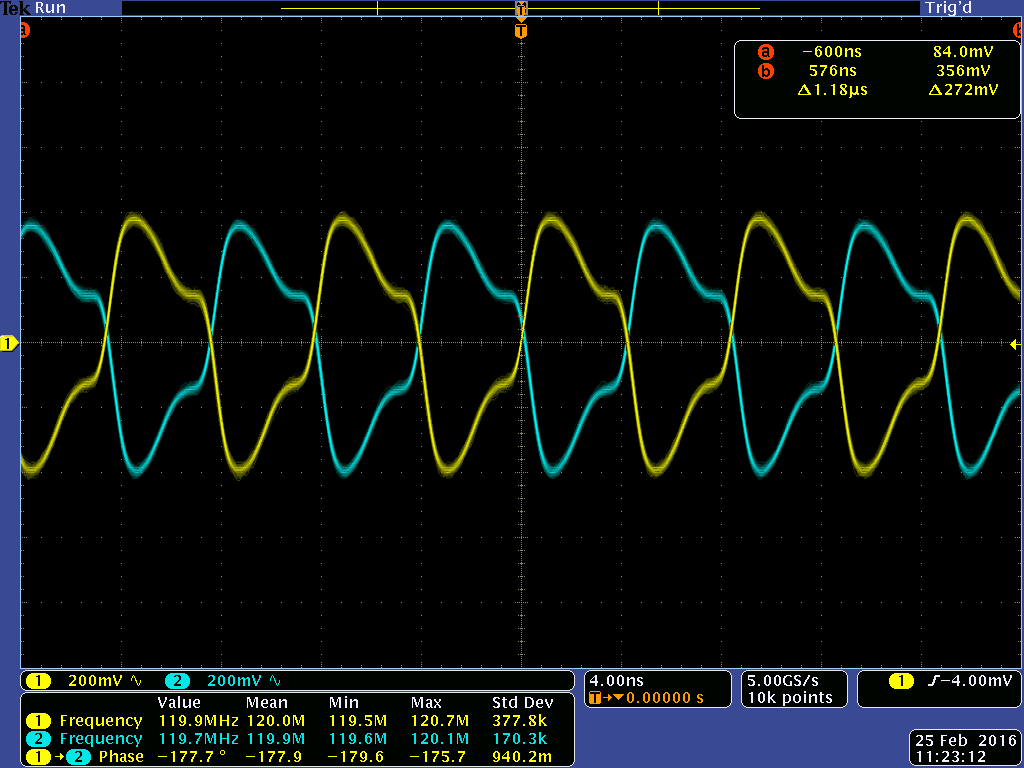
\includegraphics[scale = 0.2]{../img/20160226_tek120}}{\caption{$Si570$ After configuration: 120 MHz.}\label{fig:tek120}}
   \end{floatrow}
\end{figure}

\begin{center}
  \begin{tabulary}{1\textwidth}{|L|L|L|L|L|}
  \hline
    Index & Group & Name &  Data & Description   \\
    \hline
     P0   & \# & Latency-Optimized GBT Link - Tx                     & 0 & Low when standard GBT    \\
     \hline
     P1   & \# & Latency-Optimized GBT Link - Rx                    & 0 & Low when standard GBT      \\
     \hline
     P29 & \# & ISSP PLL Locked                                                       & 1 & Text \\
     \hline
     P3   & \# & Tx\_FrameCLK Phase Aligner - PLL Locked & 1 & Text \\     
     \hline
      S10   & \# & Tx\_FrameCLK Phase Aligner - Manual Reset & 0 & Text \\     
     \hline
      S[11..16]   & \# & Tx\_FrameCLK Phase Aligner - GBT Link 1 Steps & 0 & Each Step is 520ps \\     
     \hline
      S17   & \# & Tx\_FrameCLK Phase Aligner - Enable & 0 & Enable when ...? \\    
     \hline
      S18   & \# & Tx\_FrameCLK Phase Aligner - Trigger & 0 & Set to '1' for autoalignment. \\    
     \hline
      P4   & \# & Tx\_FrameCLK Phase Aligner - Phase Shift Done & 0 & Enabled ...? \\    
     \hline
      P2   & \# & MGT Tx PLL Locked & 1 & Text \\    
     \hline     
  \end{tabulary}  
\end{center}

\end{document}